


\tikzset{every picture/.style={line width=0.75pt}} %set default line width to 0.75pt        

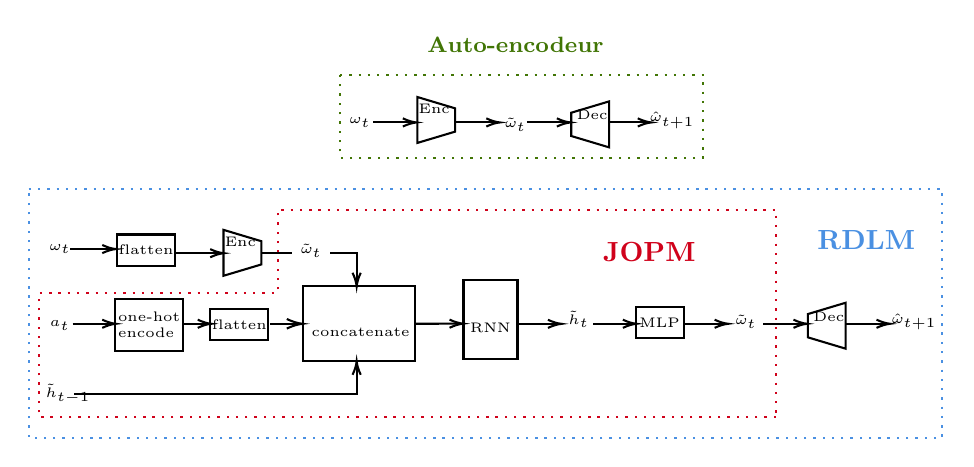
\begin{tikzpicture}[x=0.75pt,y=0.75pt,yscale=-1,xscale=1]
    %uncomment if require: \path (0,2102); %set diagram left start at 0, and has height of 2102

    %Straight Lines [id:da12291430906620326] 
    \draw    (40,1244) -- (60,1244) ;
    \draw [shift={(62,1244)}, rotate = 180] [color={rgb, 255:red, 0; green, 0; blue, 0 }  ][line width=0.75]    (6.56,-1.97) .. controls (4.17,-0.84) and (1.99,-0.18) .. (0,0) .. controls (1.99,0.18) and (4.17,0.84) .. (6.56,1.97)   ;
    %Straight Lines [id:da854600218035323] 
    \draw    (41.17,1280) -- (60,1280) ;
    \draw [shift={(62,1280)}, rotate = 180] [color={rgb, 255:red, 0; green, 0; blue, 0 }  ][line width=0.75]    (6.56,-1.97) .. controls (4.17,-0.84) and (1.99,-0.18) .. (0,0) .. controls (1.99,0.18) and (4.17,0.84) .. (6.56,1.97)   ;
    %Straight Lines [id:da8198996876977515] 
    \draw    (42,1314) -- (178,1314) -- (178,1300) ;
    \draw [shift={(178,1298)}, rotate = 90] [color={rgb, 255:red, 0; green, 0; blue, 0 }  ][line width=0.75]    (6.56,-1.97) .. controls (4.17,-0.84) and (1.99,-0.18) .. (0,0) .. controls (1.99,0.18) and (4.17,0.84) .. (6.56,1.97)   ;
    %Straight Lines [id:da16079844629341067] 
    \draw    (94,1280) -- (106,1280) ;
    \draw [shift={(108,1280)}, rotate = 180] [color={rgb, 255:red, 0; green, 0; blue, 0 }  ][line width=0.75]    (6.56,-1.97) .. controls (4.17,-0.84) and (1.99,-0.18) .. (0,0) .. controls (1.99,0.18) and (4.17,0.84) .. (6.56,1.97)   ;
    %Straight Lines [id:da8458082826263951] 
    \draw    (136.38,1280) -- (150,1280) ;
    \draw [shift={(152,1280)}, rotate = 180] [color={rgb, 255:red, 0; green, 0; blue, 0 }  ][line width=0.75]    (7.65,-2.3) .. controls (4.86,-0.97) and (2.31,-0.21) .. (0,0) .. controls (2.31,0.21) and (4.86,0.98) .. (7.65,2.3)   ;
    %Straight Lines [id:da652052323916765] 
    \draw    (90,1246) -- (112,1246) ;
    \draw [shift={(114,1246)}, rotate = 180] [color={rgb, 255:red, 0; green, 0; blue, 0 }  ][line width=0.75]    (6.56,-1.97) .. controls (4.17,-0.84) and (1.99,-0.18) .. (0,0) .. controls (1.99,0.18) and (4.17,0.84) .. (6.56,1.97)   ;
    %Shape: Trapezoid [id:dp7451370659608787] 
    \draw   (113.84,1234.74) -- (132.07,1240.21) -- (132.07,1251.42) -- (113.84,1256.88) -- cycle ;
    %Straight Lines [id:da504334878732494] 
    \draw    (132,1246) -- (178,1246) -- (178,1260) ;
    \draw [shift={(178,1262)}, rotate = 270] [color={rgb, 255:red, 0; green, 0; blue, 0 }  ][line width=0.75]    (6.56,-1.97) .. controls (4.17,-0.84) and (1.99,-0.18) .. (0,0) .. controls (1.99,0.18) and (4.17,0.84) .. (6.56,1.97)   ;
    %Straight Lines [id:da38889841564308203] 
    \draw    (206,1280) -- (227.33,1279.94) ;
    \draw [shift={(229.33,1279.94)}, rotate = 179.85] [color={rgb, 255:red, 0; green, 0; blue, 0 }  ][line width=0.75]    (6.56,-1.97) .. controls (4.17,-0.84) and (1.99,-0.18) .. (0,0) .. controls (1.99,0.18) and (4.17,0.84) .. (6.56,1.97)   ;
    %Straight Lines [id:da6070021958853442] 
    \draw    (255.89,1280.03) -- (274.72,1280.03) ;
    \draw [shift={(276.72,1280.03)}, rotate = 180] [color={rgb, 255:red, 0; green, 0; blue, 0 }  ][line width=0.75]    (6.56,-1.97) .. controls (4.17,-0.84) and (1.99,-0.18) .. (0,0) .. controls (1.99,0.18) and (4.17,0.84) .. (6.56,1.97)   ;
    %Straight Lines [id:da9474991608396127] 
    \draw    (292,1280) -- (310.83,1280) ;
    \draw [shift={(312.83,1280)}, rotate = 180] [color={rgb, 255:red, 0; green, 0; blue, 0 }  ][line width=0.75]    (6.56,-1.97) .. controls (4.17,-0.84) and (1.99,-0.18) .. (0,0) .. controls (1.99,0.18) and (4.17,0.84) .. (6.56,1.97)   ;
    %Straight Lines [id:da30117716125635063] 
    \draw    (336,1280) -- (343.4,1280) -- (355.04,1280) ;
    \draw [shift={(357.04,1280)}, rotate = 180] [color={rgb, 255:red, 0; green, 0; blue, 0 }  ][line width=0.75]    (6.56,-1.97) .. controls (4.17,-0.84) and (1.99,-0.18) .. (0,0) .. controls (1.99,0.18) and (4.17,0.84) .. (6.56,1.97)   ;
    %Shape: Trapezoid [id:dp8095835972749043] 
    \draw   (413.61,1292) -- (395.38,1286.53) -- (395.38,1275.32) -- (413.61,1269.86) -- cycle ;
    %Straight Lines [id:da826424636779827] 
    \draw    (374,1280) -- (393.04,1280) ;
    \draw [shift={(395.04,1280)}, rotate = 180] [color={rgb, 255:red, 0; green, 0; blue, 0 }  ][line width=0.75]    (6.56,-1.97) .. controls (4.17,-0.84) and (1.99,-0.18) .. (0,0) .. controls (1.99,0.18) and (4.17,0.84) .. (6.56,1.97)   ;
    %Straight Lines [id:da9956830601246753] 
    \draw    (414,1280) -- (433.04,1280) ;
    \draw [shift={(435.04,1280)}, rotate = 180] [color={rgb, 255:red, 0; green, 0; blue, 0 }  ][line width=0.75]    (6.56,-1.97) .. controls (4.17,-0.84) and (1.99,-0.18) .. (0,0) .. controls (1.99,0.18) and (4.17,0.84) .. (6.56,1.97)   ;
    %Shape: Trapezoid [id:dp7123661763765968] 
    \draw   (207.23,1170.74) -- (225.46,1176.21) -- (225.46,1187.42) -- (207.23,1192.88) -- cycle ;
    %Shape: Trapezoid [id:dp881712157773022] 
    \draw   (299.61,1195) -- (281.38,1189.53) -- (281.38,1178.32) -- (299.61,1172.86) -- cycle ;
    %Straight Lines [id:da08650198662979247] 
    \draw    (300,1183) -- (318,1183) ;
    \draw [shift={(320,1183)}, rotate = 180] [color={rgb, 255:red, 0; green, 0; blue, 0 }  ][line width=0.75]    (6.56,-1.97) .. controls (4.17,-0.84) and (1.99,-0.18) .. (0,0) .. controls (1.99,0.18) and (4.17,0.84) .. (6.56,1.97)   ;
    %Straight Lines [id:da859155317948508] 
    \draw    (186,1183) -- (204.83,1183) ;
    \draw [shift={(206.83,1183)}, rotate = 180] [color={rgb, 255:red, 0; green, 0; blue, 0 }  ][line width=0.75]    (6.56,-1.97) .. controls (4.17,-0.84) and (1.99,-0.18) .. (0,0) .. controls (1.99,0.18) and (4.17,0.84) .. (6.56,1.97)   ;
    %Straight Lines [id:da2208039710887556] 
    \draw    (226,1183) -- (245.04,1183) ;
    \draw [shift={(247.04,1183)}, rotate = 180] [color={rgb, 255:red, 0; green, 0; blue, 0 }  ][line width=0.75]    (6.56,-1.97) .. controls (4.17,-0.84) and (1.99,-0.18) .. (0,0) .. controls (1.99,0.18) and (4.17,0.84) .. (6.56,1.97)   ;
    %Straight Lines [id:da4577946170565437] 
    \draw    (260,1183) -- (279.04,1183) ;
    \draw [shift={(281.04,1183)}, rotate = 180] [color={rgb, 255:red, 0; green, 0; blue, 0 }  ][line width=0.75]    (6.56,-1.97) .. controls (4.17,-0.84) and (1.99,-0.18) .. (0,0) .. controls (1.99,0.18) and (4.17,0.84) .. (6.56,1.97)   ;
    %Shape: Polygon [id:ds4807141081631586] 
    \draw  [color={rgb, 255:red, 208; green, 2; blue, 27 }  ,draw opacity=1 ][dash pattern={on 0.84pt off 2.51pt}] (380,1325) -- (25,1325) -- (25,1265) -- (140,1265) -- (140,1225) -- (380,1225) -- cycle ;
    %Shape: Rectangle [id:dp05371260823818802] 
    \draw  [color={rgb, 255:red, 74; green, 144; blue, 226 }  ,draw opacity=1 ][dash pattern={on 0.84pt off 2.51pt}] (20,1215) -- (460,1215) -- (460,1335) -- (20,1335) -- cycle ;
    %Shape: Rectangle [id:dp09413283261737504] 
    \draw  [color={rgb, 255:red, 65; green, 117; blue, 5 }  ,draw opacity=1 ][dash pattern={on 0.84pt off 2.51pt}] (170,1160) -- (345,1160) -- (345,1200) -- (170,1200) -- cycle ;


    % Text Node
    \draw (319,1245.5) node  [color={rgb, 255:red, 208; green, 2; blue, 27 }  ,opacity=1 ] [align=left] {\textbf{JOPM}};
    % Text Node
    \draw (423.5,1239.5) node  [color={rgb, 255:red, 74; green, 144; blue, 226 }  ,opacity=1 ] [align=left] {\textbf{RDLM}};
    % Text Node
    \draw (254.5,1145.5) node  [color={rgb, 255:red, 65; green, 117; blue, 5 }  ,opacity=1 ] [align=left] {{\footnotesize \textbf{Auto-encodeur}}};
    % Text Node
    \draw (179.5,1183) node  [font=\tiny] [align=left] {$\displaystyle \omega _{t}$};
    % Text Node
    \draw (330,1182) node  [font=\tiny] [align=left] {$\displaystyle \hat{\omega }_{t+1}$};
    % Text Node
    \draw (291.5,1179.5) node   [align=left] {{\tiny Dec}};
    % Text Node
    \draw (215.38,1176.5) node   [align=left] {{\tiny Enc}};
    % Text Node
    \draw (254.5,1184) node  [font=\tiny] [align=left] {$\displaystyle \tilde{\omega }_{t}$};
    % Text Node
    \draw (446.54,1279) node  [font=\tiny] [align=left] {$\displaystyle \hat{\omega }_{t+1}$};
    % Text Node
    \draw (405.5,1276.5) node   [align=left] {{\tiny Dec}};
    % Text Node
    \draw (365.5,1279) node  [font=\tiny] [align=left] {$\displaystyle \tilde{\omega }_{t}$};
    % Text Node
    \draw (122,1240.5) node   [align=left] {{\tiny Enc}};
    % Text Node
    \draw (285,1278) node  [font=\tiny] [align=left] {$\displaystyle \tilde{h}_{t}$};
    % Text Node
    \draw    (229.48,1259) -- (255.48,1259) -- (255.48,1297) -- (229.48,1297) -- cycle  ;
    \draw (242.48,1278) node  [font=\tiny] [align=left] {\begin{minipage}[lt]{14.99pt}\setlength\topsep{0pt}
            \begin{center}
                \phantom{X}\\RNN
            \end{center}

        \end{minipage}};
    % Text Node
    \draw  [color={rgb, 255:red, 255; green, 255; blue, 255 }  ,draw opacity=1 ][fill={rgb, 255:red, 255; green, 255; blue, 255 }  ,fill opacity=1 ]  (147.5,1236) -- (164.5,1236) -- (164.5,1254) -- (147.5,1254) -- cycle  ;
    \draw (156,1245) node  [font=\tiny] [align=left] {$\displaystyle \tilde{\omega }_{t}$};
    % Text Node
    \draw    (152,1262) -- (206,1262) -- (206,1298) -- (152,1298) -- cycle  ;
    \draw (179,1280) node  [font=\tiny] [align=left] {\begin{minipage}[lt]{34pt}\setlength\topsep{0pt}
            \begin{center}
                \phantom{X}\\concatenate
            \end{center}

        \end{minipage}};
    % Text Node
    \draw    (107.5,1273) -- (135.5,1273) -- (135.5,1288) -- (107.5,1288) -- cycle  ;
    \draw (121.5,1280.5) node  [font=\tiny] [align=left] {flatten};
    % Text Node
    \draw (39,1314) node  [font=\tiny] [align=left] {$\displaystyle \tilde{h}_{t-1}$};
    % Text Node
    \draw (35,1281) node  [font=\tiny] [align=left] {$\displaystyle a_{t}$};
    % Text Node
    \draw (35,1244) node  [font=\tiny] [align=left] {$\displaystyle \omega _{t}$};
    % Text Node
    \draw    (312.5,1272) -- (335.5,1272) -- (335.5,1287) -- (312.5,1287) -- cycle  ;
    \draw (324,1279.5) node  [font=\tiny] [align=left] {MLP};
    % Text Node
    \draw    (61.5,1268) -- (94.5,1268) -- (94.5,1293) -- (61.5,1293) -- cycle  ;
    \draw (78,1280.5) node  [font=\tiny] [align=left] {one-hot\\encode};
    % Text Node
    \draw    (62.5,1237) -- (90.5,1237) -- (90.5,1252) -- (62.5,1252) -- cycle  ;
    \draw (76.5,1244.5) node  [font=\tiny] [align=left] {flatten};


\end{tikzpicture}